\documentclass[12pt,a4paper,titlepage]{article}
%%%%%%%%%%%%%%%%%%%%导言区%%%%%%%%%%%%%%%
%%宏包设置
\usepackage[BoldFont]{xeCJK}
\usepackage[dvips]{graphicx}
\usepackage[colorlinks,linkcolor=red,anchorcolor=red,citecolor=red,urlcolor=blue]{hyperref}
\usepackage{verbatim}
\usepackage{threeparttable}
%\usepackage{nl}
%%字体设置
\setCJKmainfont[BoldFont=SimHei,ItalicFont=SimSun]{SimSun}
\setmainfont{Times New Roman}
\setCJKfamilyfont{ht}{SimHei}
%%页面设置
\addtolength{\hoffset}{-1cm}
\addtolength{\voffset}{-2cm}
\addtolength{\textheight}{4cm}
\addtolength{\textwidth}{2cm}
%%标题页
\title{NIOS II Linux Tutorial}
\author{作者:陈锋\\\\审校:邢岚\\\\Email:cfistalent@gmail.com\\\\重庆大学通信工程学院2401学习资料}
%%%%%%%%%%%%%%%%%%%%正文%%%%%%%%%%%%%%%
\begin{document}
\thispagestyle{empty}
\maketitle{}
%%%%%%%%%%%%%%%%%%%%前言%%%%%%%%%%%%%%%
\section{前言}
\setcounter{footnote}{0}
本文由\LaTeX{}构建.
%源代码在\href{https://github.com/cfistalent/NiosII\_Linux\_Tutorial}{https://github.com/cfistalent/NiosII\_Linux\_Tutorial}上.
%可通过\fbox{git clone git://github.com/cfistalent/NiosII\_Linux\_Tutorial.git}获取最新的源码.

这是一个\textbf{NIOS II Linux}开发的入门教程,拟包括以下几个部分:\footnote{随着编写计划的变化,可能会有增减.}
\begin{itemize}
\item 如何获取资源;
\item 介绍\textbf{NIOS II Linux}开发环境;
\item 一个完整的流程,创建硬件到配置内核;
\item 开发前需要了解的知识;
\item linux下普通应用程序开发;
%\item linux下驱动开发举例;
\item FTK应用程序开发;
\end{itemize}
%%%%%%%%%%%%%%%%%%%%如何获得相关资料%%%%%%%%%%%%%%%
\newpage{}
\section{如何获得相关资料}
\setcounter{footnote}{0}
\subsection{网站}
\begin{description}
\item[\href{http://www.nioswiki.com/Linux}{NiosWiki上Linux主页}] 这是nios linux内核开发包的发布主页.
上面包含如何下载内核开发包,如何进行第一次编译等工作.有相应文档提供下载.
\item[\href{http://www.nioswiki.com/OperatingSystems/UClinux}{NiosWiki上uClinux主页}] 这里包含的内容大多数都适用于Linux.
因此,在动手之前请把这两个页面仔细读一读.
\item[\href{http://www.alteraforum.com/forum/forumdisplay.php?f=37}{Altera论坛}] 这里提供了一个问题交流的地方,学习过程中
遇到的问题都可以在这里获得响应.不过要注意两点:{\CJKfamily{ht}首先确认你在wiki上找不到答案,其次有合格的英语表达能力}.
\item[\href{http://sopc.et.ntust.edu.tw/pipermail/nios2-dev/}{nios linux开发者邮件列表}] 这里是nios linux的真正发源地.每个月
都会有若干个bug在这里被修复,新的版本的内核被移植.时刻关注这里可以让你与开发者同步.
\item[\href{ftp://ftp.altera.com/up/pub/}{Altera官方FTP}] 这里面资源很丰富,Altera FPGA的开发资料,Altera大学IP等等.
\item[\href{http://www.cnblogs.com/oomusou/}{一个台湾工程师的博客}] FPGA,特别是DE2和DE2-70的资源很丰富.
\item[\href{http://www.terasic.com/downloads/cd-rom/}{友晶公司的CD资源FTP}] 包含友晶公司各种开发板附带的CD资料.需要在友晶官网注册.
\end{description}
\subsection{书籍}
\begin{description}
\item[\href{http://www.amazon.cn/mn/detailApp/ref=sr\_1\_1?\_encoding=UTF8&s=books&qid=1291516849&asin=B001EJNTCC&sr=8-1}{SOPC嵌入式系统基础教程}] 介绍SOPC基础知识.是Altera官方文档的中文翻译版.有能力的同学可以直接看\href{http://www.altera.com.cn/literature/lit-nio2.jsp}{官方文档}.
\item[\href{http://www.amazon.cn/Nios-2\%E8\%BD\%AF\%E4\%BB\%B6\%E6\%9E\%B6\%E6\%9E\%84\%E8\%A7\%A3\%E6\%9E\%90-\%E8\%94\%A1\%E4\%BC\%9F\%E7\%BA\%B2/dp/B0011Y1VXO/ref=pd\_sim\_b\_2}{Nios2软件架构解析}] 将Altera的Nios2软件架构分析的很透彻,尽管针对的是6.0版本依然很有用.
\item[\href{http://www.amazon.cn/mn/detailApp/ref=sr\_1\_1?\_encoding=UTF8&s=books&qid=1291517188&asin=B004A7L87I&sr=1-1}
{Linux设备驱动开发详解}] 宋宝华老师的书,针对Linux驱动开发做了详尽的介绍.
\item[\href{http://www.amazon.cn/mn/detailApp/ref=sr\_1\_1?\_encoding=UTF8&s=books&qid=1291517330&asin=B003Q97NPC&sr=1-1}{Linux程序设计}]
 介绍Linux应用程序开发的好书.
\end{description}
%%%%%%%%%%%%%%%%%%%%构建开发环境%%%%%%%%%%%%%%%
\newpage{}
\section{构建开发环境}
\setcounter{footnote}{0}
2009年9月,nioswiki社区推出基于NIOS II处理器的linux内核开发包,为开发者提供一种新的系统方案.

使用\textbf{NIOS II Linux}开发需要搭建硬件和软件环境.目前已知的开发环境有两类:
\begin{table}[!hbtp]
\centering
\begin{tabular}{|l|p{0.68\textwidth}|}
\hline
完全在linux下开发 & 在linux下安装linux版本的Quartus II和NiosII IDE开发工具,同时安装nios-linux内核开发包.
据我所知目前只有\textbf{Ubuntu9.04}可以兼容,Ubuntu9.10及以上版本暂时不支持.\footnote{不支持的原因是nios2-download脚本在Ubuntu9.10及
以上版本中部分无法执行,而官方推荐的Redhat企业版和Fedora等均可配置}\\
\hline
WindowsXP+Linux虚拟机 & 这种方案更适合大多数平时工作在Windows环境下的开发者.本文接下来将介绍这种方案的配置.\footnote{由于在linux下
的usb-blaster驱动比windows下性能要相对差些,当构建的系统选择以JTAG-UART作为终端时,在linux环境下的"nios2-terminal"命令会导致系统阻塞,此时
我更倾向于使用本方案}\\
\hline
\end{tabular}
\caption{开发环境\label{dev_env}}
\end{table}
%%%3.1
\subsection{硬件环境}
首先需要在Windows上安装Quartus II和相应版本的NiosII IDE.本文使用是9.0版本.因此大于等于该版本都应该没有问题.
安装过程这里不赘述,有问题请自行查阅相关文档.但是安装的版本{\CJKfamily{ht}需要有lisence支持}.
%%%3.2
\subsection{软件环境}
linux内核驱动和应用程序的开发需要在类Unix操作系统下进行,最普遍的就是Linux操作系统.这里我们选择流行程度最高的Ubuntu操作系统作为开发平台.

首先我们要安装一款虚拟机软件\footnote{Windows下有Vmware,Virtual Box等}.通过该软件创建虚拟机并安装Ubuntu.安装好的虚拟机系统要满足两个要求:
\begin{itemize}
\item 能够连接互联网,下载内核开发所需的文件;
\item 能够与宿主机(Windows)交换文件.宿主机下生成的头文件要传入虚拟机中交给内核开发包使用,而虚拟机下生成的内核可执行文件要
在window下通过nios shell下载;
\end{itemize}

我们以Virtual Box为例说明如何操作\footnote{使用Vmware等只要满足上面两个条件同样可以搭建开发环境}.
%%%3.2.1
\subsubsection{虚拟机安装Ubuntu并做相关设置}
创建虚拟机之前,本地电脑上需要准备如下内容:
\begin{itemize}
\item Ubuntu安装光盘或ISO镜像文件;
\item 已安装好Virtual Box软件;
\item 足够的硬盘空间(14G左右);
\end{itemize}

在Virtual Box主页面菜单上选择\fbox{控制-->新建},操作系统类型选择\textbf{Linux},版本选择\textbf{Ubuntu},如图\ref{f_create_vb1}所示.
\begin{figure}[!bthp]
\centering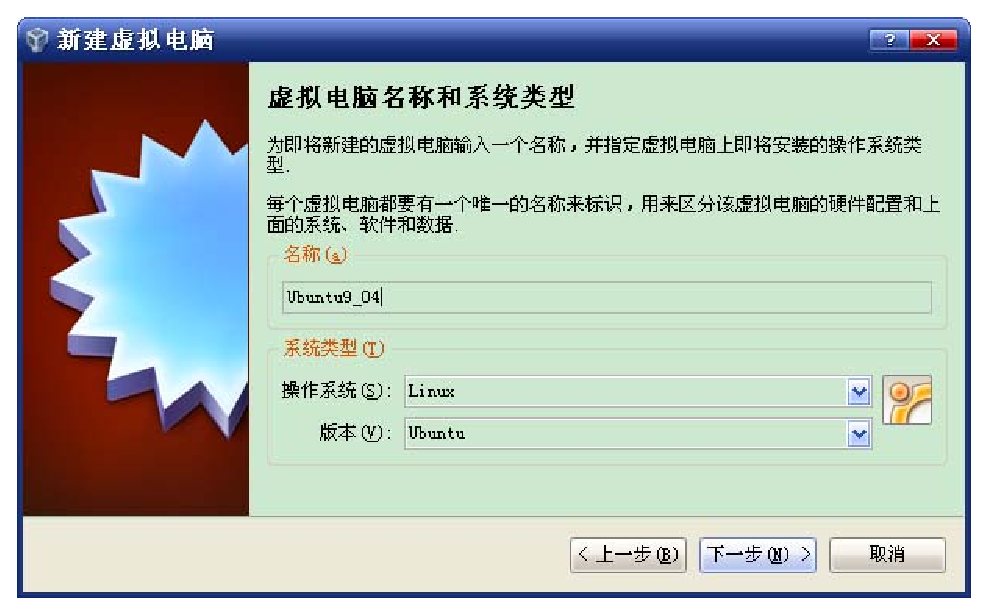
\includegraphics[width=1\textwidth]{pic/f_create_vb1.eps}
\caption{创建虚拟机:整体设定\label{f_create_vb1}}
\end{figure}
内存选择为当前系统内存一半略少,尽量发挥系统性能.硬盘选择"创建新的虚拟硬盘"并选择"固定大小"\footnote{相对于动态增长,
固定大小使得虚拟机运行速度更快}.硬盘大小至少10G,以免内核开发包在虚拟机中解压缩后空间不够,{\CJKfamily{ht}注意,默认虚拟硬盘保存在系统盘中,
请将位置改到有足够空间的磁盘上}.硬盘创建完成后确定即可.

到现在为止,虚拟机已经创建完毕.但是当前的虚拟机内没有任何系统,甚至连分区都没有,此时需要通过光驱安装操作系统.本文使用ISO镜像
文件进行安装.

在没有运行虚拟机的情况下,点击\fbox{设置}图标,右侧找到"介质"一栏,对ISO进行注册.如图\ref{iso0},\ref{iso1}和\ref{iso2}所示.
\begin{figure}[!bthp]
\centering
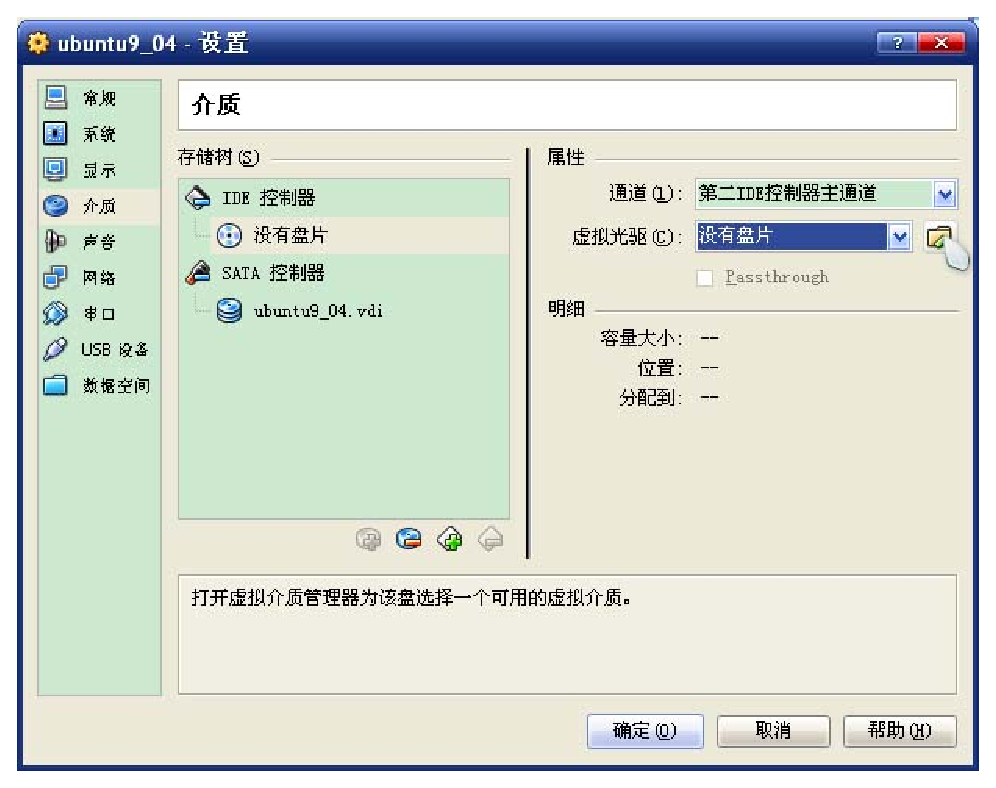
\includegraphics[width=0.8\textwidth,scale=0.8]{pic/f_vb_setting_iso.eps}
\caption{设置ISO\label{iso0}}
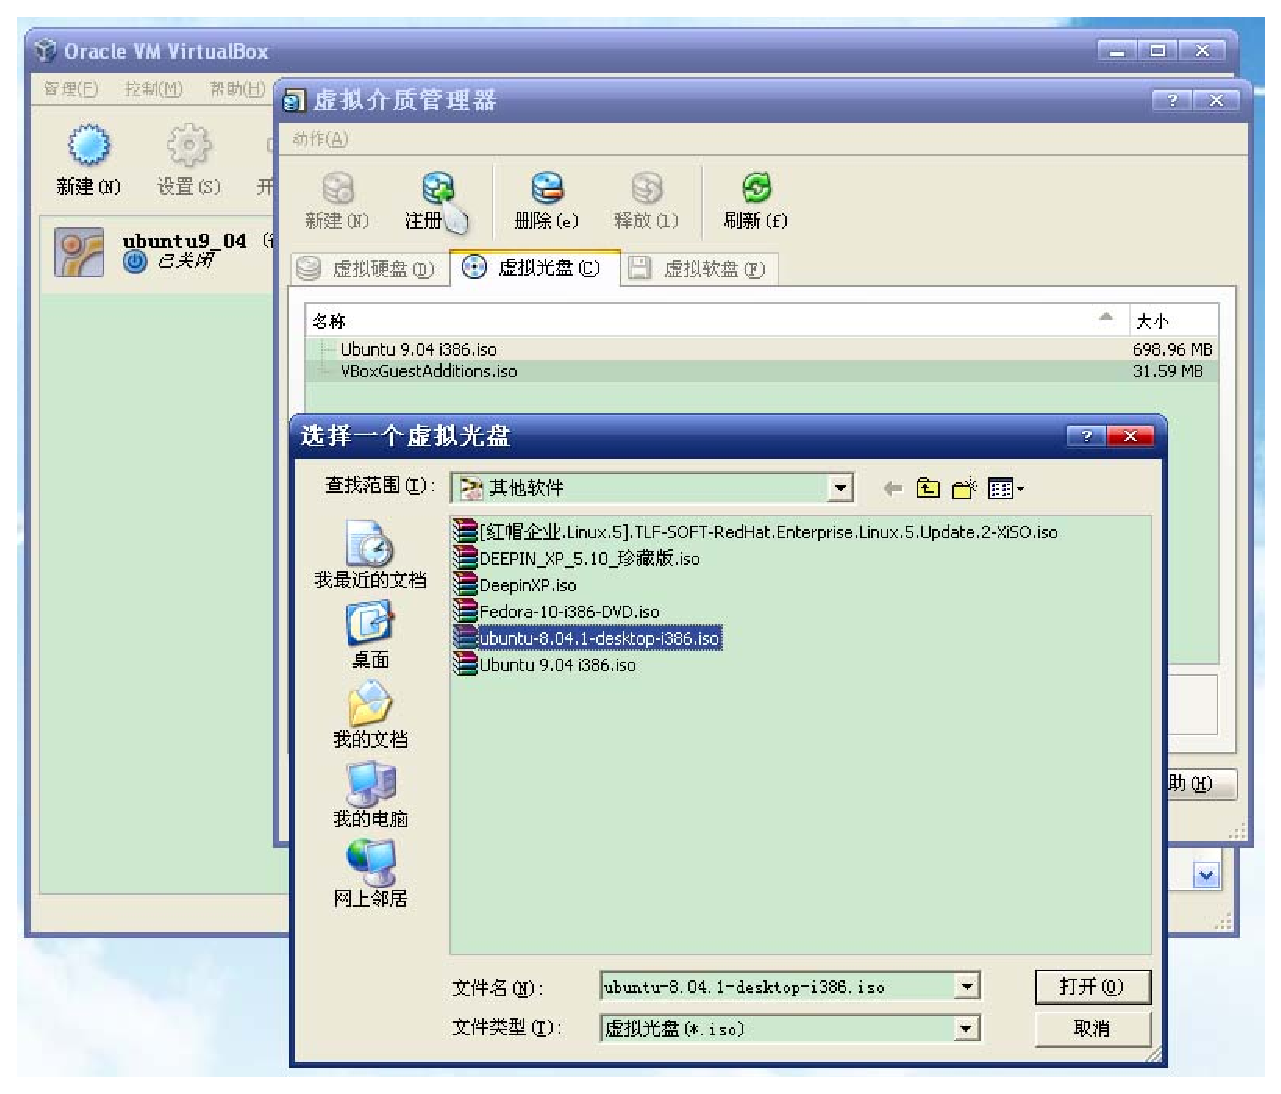
\includegraphics[width=0.8\textwidth,scale=0.8]{pic/f_vb_setting_iso_register.eps}
\caption{设置ISO\label{iso1}}
\end{figure}
\begin{figure}[!bthp]
\centering
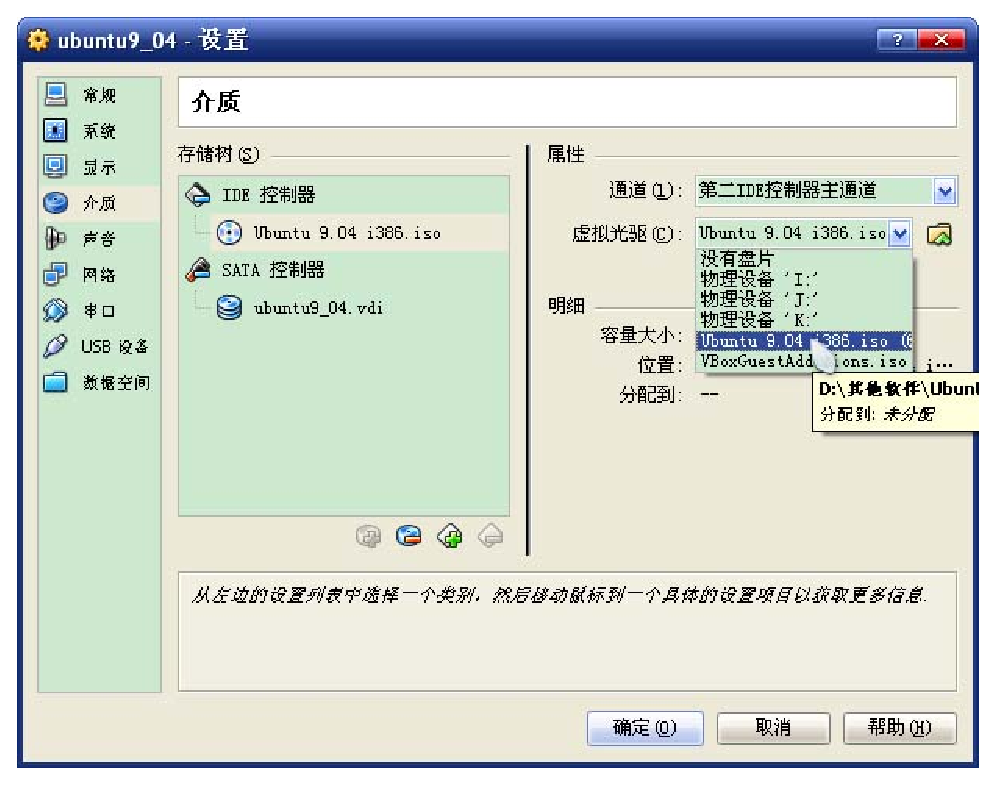
\includegraphics[width=0.8\textwidth,scale=0.8]{pic/f_vb_setting_iso_set.eps}
\caption{设置ISO\label{iso2}}
\end{figure}

之后运行虚拟机,系统就会从ISO进行引导,进而安装Ubuntu系统.过程略.

安装完成后.若宿主机能够访问互联网,则虚拟机也能访问互联网.剩下一个问题就是共享文件夹的设置.在设置之前,需要先安装Virtual Box提供的
增强工具包.在运行虚拟机的界面上选择\fbox{设备-->安装增强功能}.此时在虚拟机的桌面上就会出现一个光盘.打开终端\footnote{Alt+F2调出运行
窗口,输入\fbox{gnome-terminal}回车即可调出终端}.在终端中输入如下命令\footnote{下文中没有特别说明,运行的命令都将是在终端中}:
\begin{verse}
cd /media/cdrom\\sudo ./VBoxLinuxAdditions-x86.run \#若本地PC是amd64位架构,就运行VBoxLinuxAdditions-amd64.run\\输入管理员密码
\end{verse}
等待安装过程结束,关闭虚拟机{\CJKfamily{ht}(注意,这里一定要先关闭虚拟机)}.然后在\fbox{设置}中右侧找到"数据空间",添加一个在宿主机上已经存在的文件夹作为共享目的地.如图\ref{f_sf}所示.
启动虚拟机,终端中输入如下命令:
\begin{verse}
mkdir -p /home/<你的用户名>/Desktop/VBS \#在虚拟机中创建一个文件夹\\sudo mount -t vbox <宿主机中共享文件夹名称> 
/home/<你的用户名>/Desktop/VBS
\end{verse}
经过这番设置后,共享文件夹就设置成功了.但是,重启后设置将会失效,为使启动后系统自动处理共享文件夹,需进行如下配置.
\begin{verse}\label{cmd0}
sudo gedit /etc/fstab\\在打开的文件中添加一行" VBoxSharedFolder  /home/<你的用户名>/Desktop/VBS/  vboxsf  defaults 0 0"
\end{verse}
\begin{figure}[!bthp]
\centering
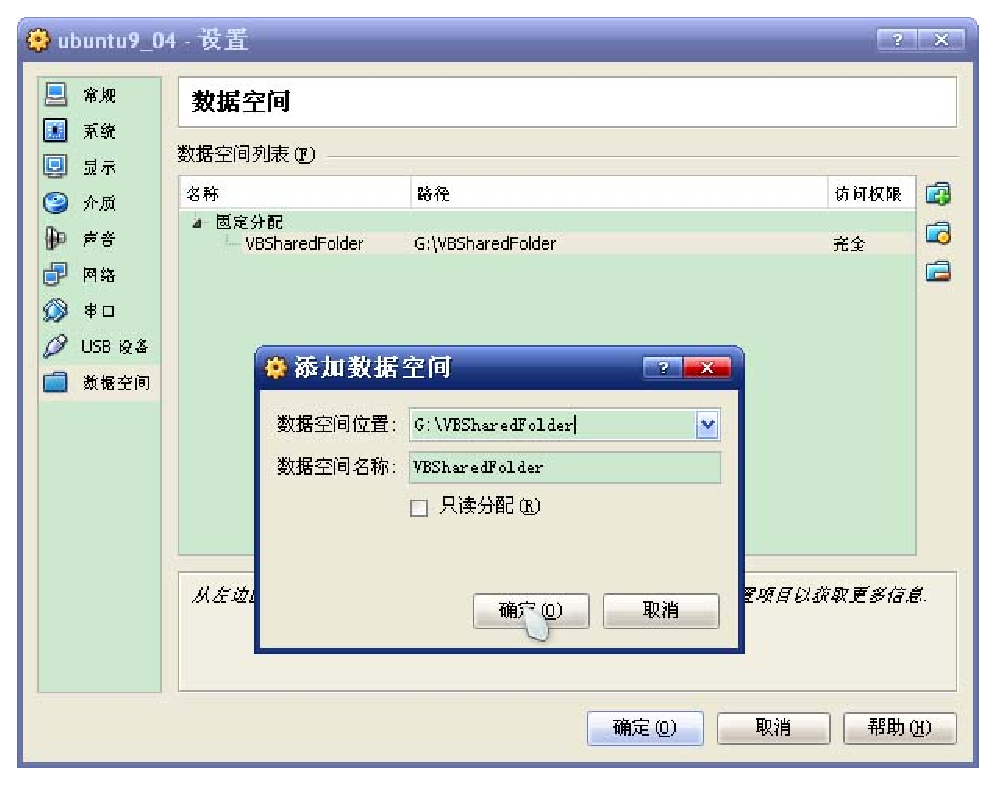
\includegraphics[width=0.8\textwidth,scale=0.8]{pic/f_vb_setting_sf.eps}
\caption{共享空间设置\label{f_sf}}
\end{figure}
%%%3.2.2
\subsubsection{内核开发包安装设置}
在安装内核开发包之前,要先安装一些基本的软件包:
\begin{verse}
sudo apt-get install git-core git-doc automake libtool enca ncurses-dev pax-utils
\end{verse}

将我提供的内核开发包\footnote{nios2-linux\_CF.tgz}拷贝到{\CJKfamily{ht}宿主机}的共享文件夹下,在{\CJKfamily{ht}虚拟机终端}运行如下命令:
\begin{verse}
cd /\\sudo chown <你的用户名,在这里,是bearchen:/> opt/\\mkdir NiosIILinux\\cd /opt/NiosIILinux/\\
tar -zxvf /home/<你的用户名>/Desktop/VBS/<内核开发包名称>
\end{verse}
我们将把内核开发不包安装在/opt目录下,前两个命令的目的是修改opt的所有者,方便之后运行命令.第三个命令则是我的内核开发包历史遗留问题.
第四个命令将内核解压缩到/opt/NiosIILinux/目录下.

{\CJKfamily{ht}注意,接下来的操作比起从官方网站下载的开发包要少一道步骤,就是将源码从git仓库中导出.因为我提供的源码包已经导出相关源码.}
接着安装内核开发所需的工具,包括gcc编译器等(其实就是将工具程序所在文件夹注册到系统环境变量中):
\begin{verse}
gedit ~/.bashrc\\在打开的文件中最后添加一行"export PATH=\$PATH:/opt/NiosIILinux/nios2-linux/toolchain-mmu/x86-linux2/bin"保存修改\\
source ~/.bashrc \#更新环境变量
\end{verse}
通过以上操作,内核开发的软件环境已经搭建完毕.为了测试当前是否搭建成功.可做如下操作:
\begin{enumerate}
\item 运行以下命令:
\begin{verse}
cd /opt/NiosIILinux/nios2-linux/uClinux-dist/\\make clean\\make menuconfig
\end{verse}
在打开的界面中\footnote{这是内核的配置菜单,在这个菜单中,Enter表示进入下一层,ESC两次表示退回上一层或者退出,SPACE表示修改选项状态}
选择"Kernel/Library/Defaults Selection--->"进入.选中"Default all settings(lose changes)".退出保存.对遇到的所有提问选择'N'.
\item 再次运行\fbox{make menuconfig}.进入"Kernel/Library/Defaults Selection--->".选中"Customize Kernel Settings".退出保存.
\item 在新弹出的配置窗口,进入"Device driver--->Network device support--->Ethernet(10 or 100mbit)--->"将"Altera Triple Speed Ethernet 
MAC Support(SLS)"选项取消.退出保存.
\item 运行以下命令\footnote{rc是linux内核启动后会自动执行的脚本文件,
可以通过他人为设置开机后自动运行的命令序列.这里设置为空,避免之后编译出的内核运行时出现不必要的现象.}:
\begin{verse}cd /opt/NiosIILinux/nios2-linux/uClinux-dist/vendors/Altera/common/\\echo > rc\end{verse}
\item 运行\fbox{make}.若接下来的过程没有错误.恭喜你.整个环境已经配置成功.
\end{enumerate}
%%%3.3
\subsection{体验NIOS II Linux}
如果你手头上正好有一块DE2-70开发板,则可以通过以下方式体验一下linux在nios处理器上运行的感觉.
\begin{enumerate}
\item 找到本文附带的文件夹中的两个文件"Starter\_Hardware.sof"和"Starter\_Kernel.gz".将他们拷贝到同一个文件夹下.
\item 运行nios shell.如图\ref{ns}所示.
\item 将DE2-70的电源和usb-blaster连接好.上电.
\item 在nios shell下进入刚才保存两个文件的目录.{\CJKfamily{ht}运行命令}\footnote{注意,这里是在宿主机的nios shell下输入命令}:
\begin{verse}
nios2-config-sof Starter\_Hardware.sof\ {}\ {}\&\&\ {}\ {}nios2-download -g Starter\_Kernel.gz\ {}\ {}\&\&\ {}\ {}nios2-terminal
\end{verse}
在nios shell上打印一堆信息后将看到类似终端的命令提示符.
若一切正常,此时的nios shell将作为开发板上运行的linux内核的终端与用户交互,你可以尝试输入命令获得响应.
\end{enumerate}
\begin{figure}[!htbp]
\centering
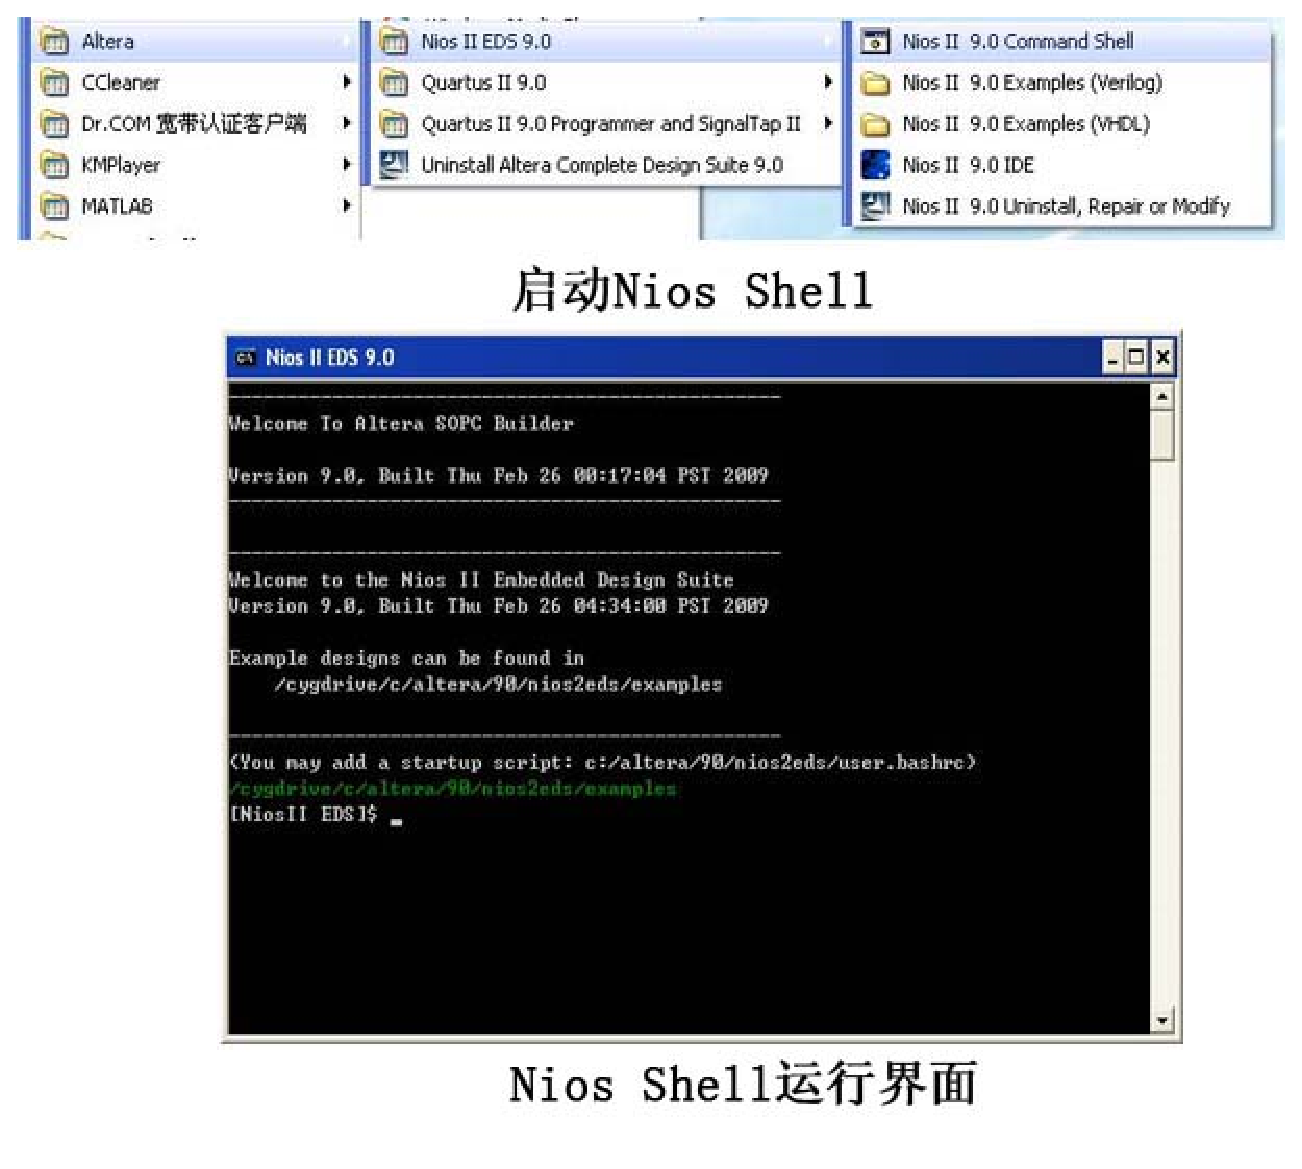
\includegraphics[width=0.75\textwidth,scale=0.75]{pic/f_shell_and_icon.eps}
\caption{Nios Shell图标和运行界面\label{ns}}
\end{figure}
%%%%%%%%%%%%%%%%%%%%走一遍流程%%%%%%%%%%%%%%%
\newpage{}
\section{第一个工程}
\setcounter{footnote}{0}
阅读本节内容的前提是读者已了解Quartus II和SOPC Builder的使用方法.否则请自行学习相关内容.

本节通过一个简单工程介绍整个设计流程.使用的硬件是\textit{DE2-70}\footnote{使用其他开发板一样可以完成本节内容,只需要
满足NiosII Linux开发的硬件最低要求}.整个过程包括但不限于:{\CJKfamily{ht}SOPC构建,顶层模块设计及管脚分配,linux内核
简单配置,下载运行}.
%%%4.1
\subsection{硬件设计}
构建的片上系统必须满足以下几个硬性条件,才能够运行linux内核和应用程序:
\begin{itemize}
\item FPGA芯片至少是Cyclone\footnote{这是基于当前开发社区提供资料的推测};
\item cpu类型至少是标准型(s),快速型(f)更佳;
\item 内存至少为8MB;
\item 必须有一个全功能定时器外设(timer),定时时间为10ms;
\item 必须有一个linux内核与外界交互的终端.一般为JTAG-UART或者UART;
\end{itemize}

\begin{enumerate}
\item 使用Quartus II的工程创建向导新建一个工程.启动SOPC Builder\footnote{{\CJKfamily{ht}接下来所有组件的设置,对没有提到的参数,
一律为默认设置}},添加CPU,{\CJKfamily{ht}无视错误信息},先保存.
添加一个SDRAM Controller.存储器设置内容\footnote{相关信息根据\textit{DE2-70}开发板上SDRAM
参数填写.其他开发板请查阅相应SDRAM数据手册}:
\begin{table}[!bhtp]
\centering
\begin{tabular}{|c|c|c|c|c|c|}
\hline
Presets & Data Width & Chip select & Banks & Row & Column \\
\hline
Custom & 16 & 1 & 4 & 13 & 9\\
\hline
\end{tabular}
\caption{SDRAM Controller:Memory Profile}
\end{table}
\begin{table}[!bhtp]
\centering
\begin{tabular}{|l|c|}\hline
CAS latency cycles & 3\\\hline
Initialization refresh cycles & 2\\\hline
Issue one refresh command every & 7.8125 us\\\hline
Delay after powerup,before initialization & 200us\\\hline
Duration of refresh command(t\_rfc) & 70ns\\\hline
Duration of precharge command(t\_rp) & 20ns\\\hline
ACTIVE to READ or WRITE delay(t\_rcd) & 20ns\\\hline
Access time(t\_ac) & 5.5ns\\\hline
Write recovery time(t\_wr,no auto precharge) & 14ns\\\hline
\end{tabular}
\caption{SDRAM Controller:Timing}
\end{table}
\\保存为默认名称\textbf{"sdram\_0"}.
\item 为了使用CPU的MMU功能,需要添加一个onchip memory,需要配置的内容:类型为\textbf{RAM},\textbf{Dual-port access},
内存大小\textbf{1024 Bytes}.其他配置默认.名称没有指定,只要有意义即可.
\item 打开CPU配置界面,Reset Vector和Exception Vector都选为\textbf{sdram\_0}.Exception Vector的偏移地址选为\textbf{0x20}.
钩选\textbf{"Include MMU"},Fast TLB Exception Vector选为刚才添加的onchip memory.偏移量为\textbf{0}.在CPU的"Caches and Memory interfaces"
选项卡中,钩选\textbf{"Include tightly coupled instruction master port(s)"}和
\textbf{"Include tightly coupled data master port(s)"}.在"JTAG Debug Module"选项卡中,
将JTAG选为\textbf{level 2}.其余选项均默认.确定退出CPU设置.对cpu和sdram controller以及onchip memory
作图\ref{f_cpu_sdram_tcm}方式连接.
\begin{figure}[!bhtp]
\centering
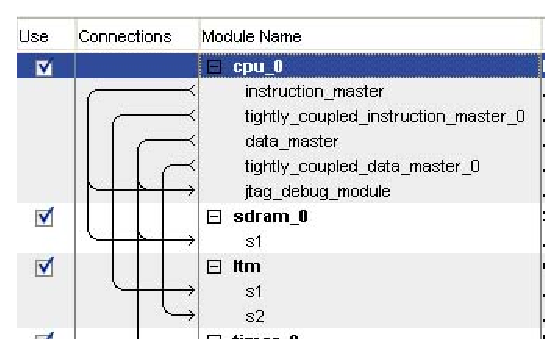
\includegraphics[width=0.6\textwidth]{pic/f_sopc_cpu_tcm_sdram.eps}
\caption{CPU与SDRAM Controller以及Fast FLB连接方式\label{f_cpu_sdram_tcm}}
\end{figure}
\item 添加一个Interval Timer作为linux内核的系统时钟.周期设为\textbf{10 ms},计数器位宽\textbf{32 bit},Presets为\textbf{Full-featured}.
\underline{{\CJKfamily{ht}timer的中断优先级一定设置为0}}.
\item 添加一个JTAG-UART,默认设置.
\item 添加一个UART,默认设置.
\item 以上构成了linux运行所需的最小配置(严格来说,JTAG-UART和UART可以只选一个,但必须有).\textit{DE2-70}上晶振为50Mhz,
为提高系统运行速度,我们添加一个PLL,运行ALTPLL MegaWizard,启用两个输出c0和c1.将c0输出为输入的一倍(100Mhz),其余值默认.
将c1输出也设置为输入的一倍(100Mhz).唯一不同的是,c1的Clock phase shift设置为\textbf{-65 deg}.
\item 修改SOPC系统中每一个组件的时钟,除了PLL是默认的外部输入时钟外,其余均改为pll\_c0时钟.
\item 点击System菜单下的Auto-Assign Base Address自动分配各组件基址以消除地址冲突.注意Auto-Assign IRQs这个选项很可能会将timer的优先级
修改,如果使用,请一定小心.完成后SOPC Builder界面如图\ref{f_sopc}所示.保存当前设置.点击Generate生成SOPC系统.
\begin{figure}[!bthp]
\centering
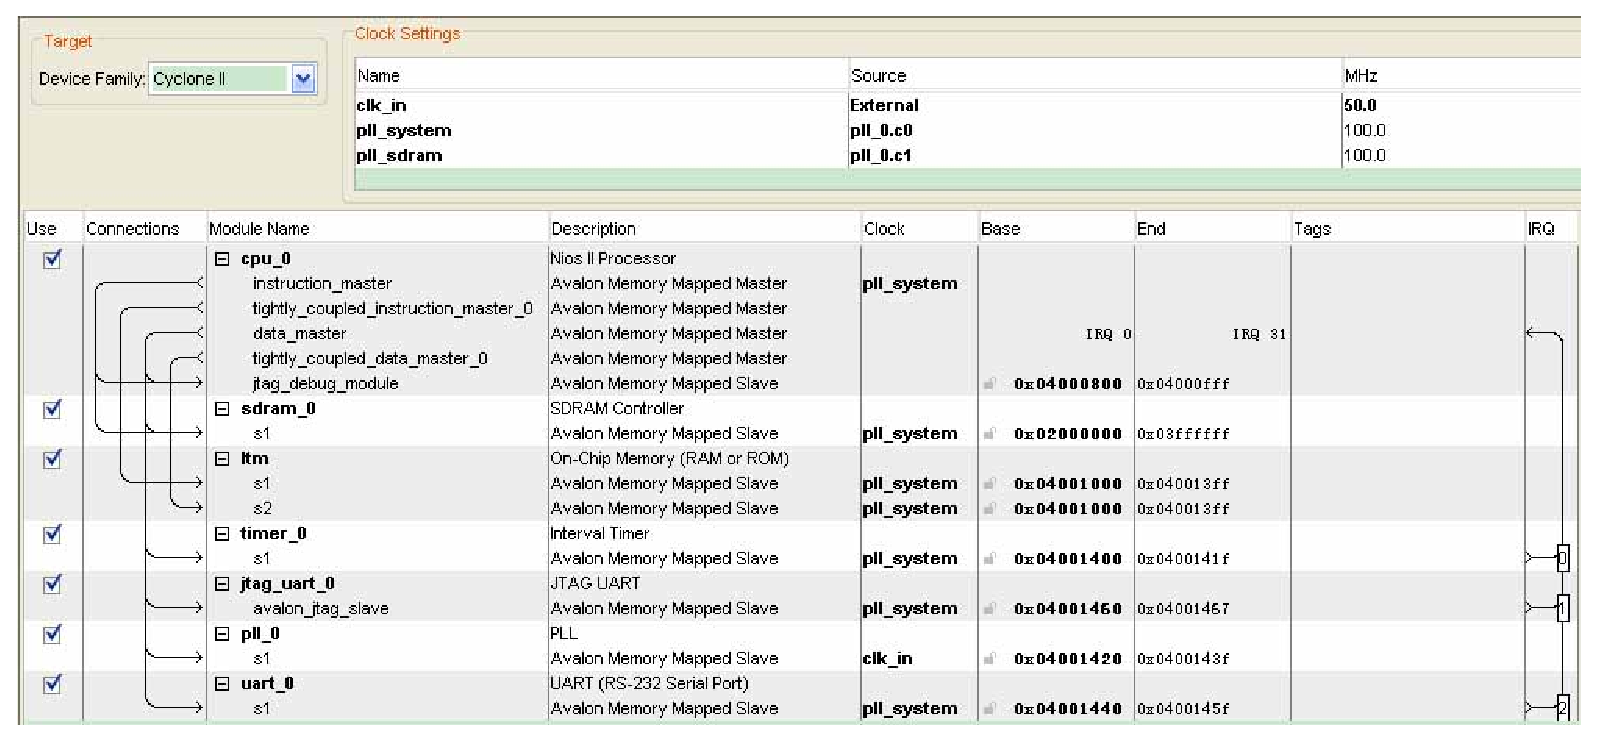
\includegraphics[width=1\textwidth]{pic/f_sopc.eps}
\caption{完成设置的SOPC\label{f_sopc}}
\end{figure}
\item 在Quartus II下新建一个.v文件作为顶层文件\footnote{顶层模块名称,保存.v文件时文件名必须与该名称一致}.添加如下内容:
\begin{verbatim}
module NL(
  input         iCLK_50,        // 50 MHz
  //////////////////////////////// UART ////////////////////////////
  output        oUART_TXD,      // UART Transmitter
  input         iUART_RXD,      // UART Receiver
  //////////////////////////////// SDRAM Interface ////////////////////////
  inout  [31:0] DRAM_DQ,        // SDRAM Data bus 32 Bits
  output [12:0] oDRAM0_A,       // SDRAM0 Address bus 12 Bits
  output        oDRAM0_LDQM0,   // SDRAM0 Low-byte Data Mask 
  output        oDRAM0_UDQM1,   // SDRAM0 High-byte Data Mask
  output        oDRAM0_WE_N,    // SDRAM0 Write Enable
  output        oDRAM0_CAS_N,   // SDRAM0 Column Address Strobe
  output        oDRAM0_RAS_N,   // SDRAM0 Row Address Strobe
  output        oDRAM0_CS_N,    // SDRAM0 Chip Select
  output [1:0]  oDRAM0_BA,      // SDRAM0 Bank Address
  output        oDRAM0_CLK,     // SDRAM0 Clock
  output        oDRAM0_CKE      // SDRAM0 Clock Enable
);
wire CPU_CLK;
wire SYS_RESET_N;
assign SYS_RESET_N=1'b1;
Nios nios2 (
  .clk_in(iCLK_50),
  .pll_system(CPU_CLK),
  .pll_sdram(oDRAM0_CLK),
  .reset_n(SYS_RESET_N),
  .zs_addr_from_the_sdram_0(oDRAM0_A),
  .zs_ba_from_the_sdram_0(oDRAM0_BA),
  .zs_cas_n_from_the_sdram_0(oDRAM0_CAS_N),
  .zs_cke_from_the_sdram_0(oDRAM0_CKE),
  .zs_cs_n_from_the_sdram_0(oDRAM0_CS_N),
  .zs_dq_to_and_from_the_sdram_0(DRAM_DQ),
  .zs_dqm_from_the_sdram_0({oDRAM0_UDQM1,oDRAM0_LDQM0}),
  .zs_ras_n_from_the_sdram_0(oDRAM0_RAS_N),
  .zs_we_n_from_the_sdram_0(oDRAM0_WE_N),
  .rxd_to_the_uart_0(iUART_RXD),
  .txd_from_the_uart_0(oUART_TXD)
);
endmodule
\end{verbatim}
其中,Nios是构建的SOPC名称.将该文件设置为顶层文件.进行编译.编译结束后,查询\textit{DE2-70}数据手册,分配顶层各信号管脚.
再进行一次编译.整个硬件系统就搭建完毕.
\end{enumerate}
%%%4.2
\subsection{内核配置和编译}
现在我们来配置当前SOPC系统对应的linux内核.
\begin{enumerate}
\item 打开nios shell(如图\ref{ns}所示),进入到硬件工程所在目录下,运行:
\begin{verse}
sopc-create-header-files --single custom\_fpga.h\footnote{生成的头文件名字一定为\textbf{custom\_fpga.h}}
\end{verse}
这将会在该目录下生成名为\textbf{custom\_fpga.h}的C语言头文件.将这个文件拷贝到共享文件夹当中.
\item 启动虚拟机,输入如下命令:
\begin{verse}
cp -i /home/bearchen\footnote{这是我的Ubuntu虚拟机下用户名,请替换成你自己的用户名}/Desktop/VBS\footnote{这是我的共享文件夹名称,同样
请替换成你的}/custom\_fpga.h /opt/NiosIILinux/nios2-linux/linux-2.6/arch/nios2/include/asm/\\
确认替换当前已有文件
\end{verse}
\item 输入命令:
\begin{verse}
cd /opt/NiosIILinux/nios2-linux/uClinux-dist/\\
make clean\\
make menuconfig\\
\end{verse}
进入内核配置界面.由于本系统比较简单,除了JTAG-UART和UART外没有任何外设,因此内核中设备驱动部分只需设置两种串口驱动支持以及
哪一种设备作为终端输出.但是,有一些设置虽然只需配置一次,但影响全局,需要特别注意.为介绍整个过程,我们先将当前配置除去.
选择"Kernel/Library/Defaults Selection--->"进入.选中"Default all settings(lose changes)".退出保存.对遇到的所有提问选择'N'.将整个内核包
恢复到默认发布配置.
\item 再次运行\fbox{make menuconfig}.进入"Kernel/Library/Defaults Selection--->".选中"Customize Kernel Settings".退出保存.
\item 在新弹出的配置窗口,进入"NiosII Configuration--->",将"NiosII FPGA Configuration(MMU\_DEFAULT)"修改为"NiosII FPGA Configuration
(CUTOM\_FPGA)"
\item 在同一个窗口中将"Link address offset fot booting"的值改大,防止内核解压缩后的代码覆盖压缩内容,这里改为\textbf{0x00F00000}.
\item 退出到上一个界面,进入"Device driver--->Network device support--->Ethernet(10 or 100mbit)--->"将"Altera Triple Speed Ethernet 
MAC Support(SLS)"选项取消\footnote{开发包默认使用Stratix的开发板和这一款网络驱动,与本工程不符.若不取消,编译报错.}.退出保存.
\item 退回到"Device driver--->"下,进入"Character devices--->Serial drivers".选择JTAG-UART和UART驱动支持,并开启JTAG-UART终端(console)支持.
如图\ref{f_kcfg_ct}所示.设置完成,退出并保存.
\begin{figure}[!bhtp]
\centering
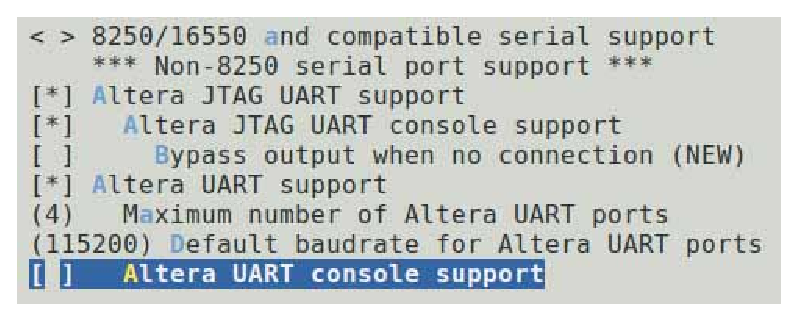
\includegraphics[width=0.6\textwidth]{pic/f_kcfg_char_terminal.eps}
\caption{内核配置:终端配置\label{f_kcfg_ct}}
\end{figure}
\item 运行\fbox{make}.内核编译完成.将images/zImage.initramfs.gz拷贝到共享文件夹\footnote{{\CJKfamily{ht}共享文件夹是联系宿主机和
虚拟机的通道,在宿主机和虚拟机中都有一个相应的文件夹进行关联}}中.
\end{enumerate}
%%%4.3
\subsection{下载运行}
此时在宿主机的共享文件夹中就存在有从虚拟机拷贝出来的内核镜像文件,为了让linux在开发板上跑起来,需要按顺序下载{\CJKfamily{ht}硬件sof文件,
内核镜像文件}.

下载sof文件有两种方法,一种是在Quartus II中直接调用Programmer下载,另一种通过nios shell下调用命令来进行.这里采用第二种.将硬件sof文件和
内核文件拷贝到同一个文件夹下.连接好\textit{DE2-70}开发板的下载线和电源,上电,在nios shell下进入该文件夹,运行如下命令:
\begin{verse}
nios2-config-sof <sof文件> \&\& nios2-download -g <内核镜像文件> \&\& nios2-terminal
\end{verse}
下载完成后,将会看到大量的打印信息,最终在shell上会出现类似Ubuntu下终端提示符的界面,如图\ref{f_kb}所示.你可以输入ls命令查看当前开发板上的
文件系统,进入/bin目录运行可执行文件等.当你执行这些操作时,恭喜你,linux已经在开发板上跑起来了.
\begin{figure}[!bhtp]
\centering
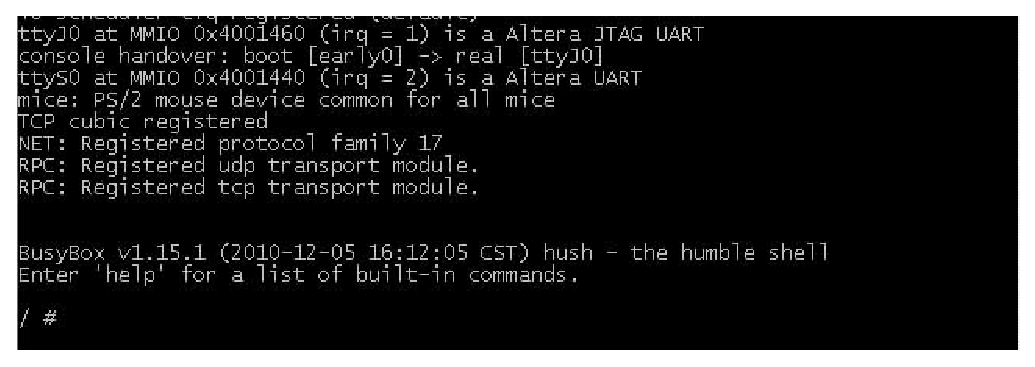
\includegraphics[width=0.8\textwidth]{pic/f_kernel_bootingmsg.eps}
\caption{内核启动完成\label{f_kb}}
\end{figure}

提醒:对于入门的同学,掌握整个开发流程是必要的;而对于进行大规模系统开发的同学,建议使用模板进行修改,效率会得到很大的提高.
%%%%%%%%%%%%%%%%%%%%开发前需要了解的知识%%%%%%%%%%%%%%%
\newpage{}
\section{开发前需要了解的知识}
\setcounter{footnote}{0}
本节将介绍一些开发所需要的背景知识,但不会进行深入的讨论.一来笔者本身也只留于表面;二来有违本文宗旨,且篇幅不允许.

通过上一节的例子,读者应该对NIOS II Linux系统开发的基本步骤有了大概的认识.至于每一步的目的是什么恐怕会有许多迷惑.本节将对内核开发中的若干
问题进行解释.纯属个人理解,水平有限,如有不对的地方,欢迎同学与我\href{mailto:cfistalent@gmail.com}{联系}.
%%%5.1
\subsection{内核开发包目录结构}
解压完内核开发包,生成名为"nios-linux"的文件夹,进入该文件夹,可以看到有如下内容:
\begin{quote}
3c120\_default binutils checkout elf2flt gcc3 glibc insight\\
linux-2.6 README sshkey toolchain-build toolchain-mmu\\
u-boot uClibc uClinux-dist update use\_git\_for\_update\\
use\_http\_for\_update use\_ssh443\_for\_update
\end{quote}
其中有几个比较重要:
\begin{description}
\item[\textit{linux-2.6}] 保存了linux内核的所有相关代码,其中大部分是各种驱动程序.驱动程序移植和开发工作都将在这个目录下
的driver目录中进行.同时arch/nios目录下保存有nios处理器相关的底层代码,包括各种片上系统对应的头文件,内核启动代码,各种片上外设的配置等.
\item[toolchain-mmu] 存有nios linux开发工具集,包括gcc,gdb等.
\item[u-boot] 存有引导linux操作系统的著名的bootloader.
\item[glibc] nios linux下开发应用程序所采用的标准C语言库函数.
\item[\textit{uClinux-dist}] 这是开发时大部分时间都将要驻留的文件夹,在这个文件夹中,有nios linux下应用程序开发时使用的各种库函数
,也有已经移植到nios linux下的各种应用程序,二者都以源码的形式存放在这个文件夹的lib和user文件夹中.
同时,这里也是运行内核配置,编译内核等命令的目录.随后我会作进一步介绍.
\item[uClibc] 内核开发包中其实包含了两个操作系统源码,带MMU的nios处理器支持的linux和不带MMU的nios处理器支持的uClinux.而uClibc就是
uClinux系统下C语言的标准函数库.两个操作系统源码存在于git\footnote{Linus开发的一个分布式版本管理系统}的两个不同分支中,
通过\fbox{git checkout}命令切换.
\item[checkout] 这是一个shell脚本,通过该脚本可利用git更新本地各个文件夹源码的版本.
\end{description}

nios linux内核开发包中,除了移植到nios处理器上的linux内核代码,还包含有大量应用程序库函数和各种应用程序的源代码,通过配置菜单决定
每个函数库和应用程序是否被编译,生成的应用程序是否会放入RAM文件系统中.这些库和程序都在uClinux-dist文件夹中.

进入uClinux-dist,有如下内容:
\begin{quote}
auto.conf  config         images       Makefile     release\_notes  tools
autoconf.h  config.arch    Kconfig      Makefile.am  romfs          user
bfin\_patch  COPYING        lib          Makefile.in  SOURCE         vendors
bin         Documentation  linux-2.6.x  openswan     staging
ccache      freeswan       MAKEALL      README       testsuites
\end{quote}
其中有几个比较重要:
\begin{description}
\item[images] 编译内核生成的可执行文件会被放到这个文件夹中.
\item[romfs] 用来生成RAM文件系统的暂存文件夹,nios linux运行时文件系统中的所有文件都来自这里.因此,如果有自定义的文件
需要放置到文件系统中,可将其放入本文件夹,运行\fbox{make romfs}即可.
\item[user] 这里有各种应用程序,如web服务器,网络工具,磁盘工具等linux应用程序.我们自行编写的应用程序也将放在这里.
\item[lib] 这里有各种函数库,如jpeg编解码库,触摸屏设备坐标提取库等等.
\item[vendors] 里面是以公司或产品为名称的文件夹,包含有针对各款产品移植的linux对应的配置文件,如设备文件,shell初始化完毕后执行的脚本文件
等等.nios linux只与"Altera"和"Generic"两个文件夹相关.
\item[staging] user中的应用程序大部分都依赖lib里的函数库,编译过程也是先lib再user,为了编译user中的应用程序时编译器能找到对应的依赖库函数
和头文件,编译完lib后会将其中的.a,.so以及.h文件拷贝到staging中,方便user的编译过程.
\end{description}

这里解释一下什么是RAM文件系统.在以nios为中心的嵌入式系统中,硬盘和大容量flash不是必须组件,因此,linux运行所需的文件系统需要放在一个必须存在
的组件当中.而内存无论以onchip ram,sdram还是sram的形式存在,都是nios嵌入式系统必须的,故内核开发包中构建了ram filesystem.生成的内核可执行
文件中,名为"zImage.initramfs.gz"的镜像包含了linux内核以及RAM文件系统.上电运行时,解压缩代码将会把内核和文件系统解压缩到指定的内存地址当中.

内核以Kconfig文件管理所有组件是否被编译,以makefile文件管理编译过程."config/.config"文件包含当前应用层配置情况(包括函数库和应用程序),
"linux-2.6.x/.config"包含当前linux内核配置情况.可通过备份这两个文件保存当前配置.
%%%5.2
\subsection{三个重要的文件}
构建SOPC系统的时候,可以添加各种外设,如uart,spi,gpio等.这些外设的名称又因人而异,而内核中,典型外设的驱动是支持的,比如串口.如何让驱动程序
支持不同设计者构建的SOPC系统?碰到内核不支持的驱动如何处理?这是本小节需要解释的内容.

内核开发包的linux源码中已支持多种设备驱动,绝大多数SOPC外设对应的驱动程序都属于"platform driver".每一个"platform driver"都有一个
"platform device"相对应\footnote{linux内核初始化过程中,会先注册若干"platform device",之后编译进内核的"platform driver"将会匹配已注册
的平台设备,若匹配成功,则利用平台驱动初始化该设备.}.在"<内核开发包路径>/nios2-linux/linux-2.6/arch/nios2/kernel"中,有一个名为
\textbf{config.c}的文件,这个文件部分内容如下所示:
\begin{verbatim}
/*Altera JTAG UART*/
#if defined(CONFIG_SERIAL_ALTERA_JTAGUART)
static struct altera_jtaguart_platform_uart nios2_jtaguart_platform[] = {
#ifdef JTAG_UART_BASE
	{
	 .mapbase = JTAG_UART_BASE,
	 .irq = JTAG_UART_IRQ,
	 },
#endif
	{},
};

static struct platform_device nios2_jtaguart = {
	.name = "altera_jtaguart",
	.id = 0,
	.dev.platform_data = nios2_jtaguart_platform,
};
#endif
/*Altera UART*/
#if defined(CONFIG_SERIAL_ALTERA_UART)
static struct altera_uart_platform_uart nios2_uart_platform[] = {
#ifdef UART_0_BASE
	{
	 .mapbase = UART_0_BASE,
	 .irq = UART_0_IRQ,
	 .uartclk = UART_0_FREQ,
	 },
#endif
	.......
	.......
	{},
};
static struct platform_device nios2_uart = {
	.name = "altera_uart",
	.id = 0,
	.dev.platform_data = nios2_uart_platform,
};
#endif
\end{verbatim}
可以看到,其中使用了很多宏定义,形如CONFIG\_XXXX的宏来自Kconfig配置生成的头文件.而其他宏则来自custom\_fpga.h文件
(在"<内核开发包路径>/nios2-linux/linux-2.6/arch/nios2/include/asm"中,后面要介绍的\textbf{nios.h}也来自该路径).

config.c中定义了很多平台设备,如uart,jtag-uart,mmc spi,dm9000等等.他们都通过一个条件编译宏指令控制是否参与最终的编译.以UART为例,
当定义了\textbf{UART\_0\_BASE}时,对应平台设备的参数如.mapbase等就会得到配置.linux支持四个串口设备,因此如果分别定义了
\textbf{UART\_1\_BASE,UART\_2\_BASE,UART\_3\_BASE},则将会有四个串口平台设备得到注册.

从另一个角度说,若config.c中没有开启某个宏进行平台设备注册,则该设备的平台驱动编译进内核后初始化时将找不到匹配设备\footnote{仅适用于
平台设备和平台驱动}.

nios.h定义了一个系统的基础组件如内存基址和大小,定时器设置以及作为系统终端的UART和JTAG-UART的设备基址等.同时还定义了nios中断号等
系统关键内容.该文件部分内容如下所示:
\begin{verbatim}
#if defined(CONFIG_NIOS2_DEFAULT_MMU)
#include <asm/default_mmu.h>
#elif defined(CONFIG_NIOS2_MAXIMUM_MMU)
#include <asm/maximum_mmu.h>
#elif defined(CONFIG_NIOS2_CUSTOM_FPGA)
#include <asm/custom_fpga.h>
#else
#error "No FPGA configuration selected
#endif

/* 2C35 dev board */
#ifdef TIMER_0_FREQ

#define CONFIG_ALTERA_CYCLONE_II
#define DDR2_TOP_BASE SDRAM_0_BASE
#define DDR2_TOP_SPAN (SDRAM_0_SPAN)

#define TIMER_1MS_FREQ TIMER_0_FREQ
#define TIMER_1MS_BASE TIMER_0_BASE
#define TIMER_1MS_SPAN TIMER_0_SPAN
#define TIMER_1MS_IRQ TIMER_0_IRQ

#define UART_BASE UART_0_BASE
#define UART_SPAN UART_0_SPAN
#define UART_IRQ UART_0_IRQ
#define UART_FREQ UART_0_FREQ

#define JTAG_UART_BASE JTAG_UART_0_BASE
#define JTAG_UART_SPAN JTAG_UART_0_SPAN
#define JTAG_UART_IRQ JTAG_UART_0_IRQ

#endif
\end{verbatim}
可以看到,针对不同的系统配置,该文件将会包含不同的头文件.这就解释了之前在进行第一个工程内核配置操作中为何要选择"CONFIG\_NIOS2\_CUSTOM\_FPGA"
.由该文件内容可以看到,这些系统基本组件的名称是固定的,如串口基址为UART\_0\_BASE.这些被替代的宏都来自于用户设计SOPC所生成的.C头文件
\textbf{custom\_fpga.h}.

现在,我们再看看上一节中生成的custom\_fpga.h的部分内容:
\begin{verbatim}
#define CPU_IMPLEMENTATION "fast"
#define CPU_FREQ 100000000u
#define ICACHE_LINE_SIZE 32
#define ICACHE_LINE_SIZE_LOG2 5
#define ICACHE_SIZE 4096
#define DCACHE_LINE_SIZE 32
#define DCACHE_LINE_SIZE_LOG2 5
#define DCACHE_SIZE 2048
......
#define MMU_PRESENT 
#define KERNEL_REGION_BASE 0xc0000000
#define IO_REGION_BASE 0xe0000000
#define KERNEL_MMU_REGION_BASE 0x80000000
#define USER_REGION_BASE 0x0
......
#define EXCEPTION_ADDR 0xc2000020
#define RESET_ADDR 0xc2000000
#define BREAK_ADDR 0xc4000820
......
#define SDRAM_0_COMPONENT_TYPE altera_avalon_new_sdram_controller
#define SDRAM_0_COMPONENT_NAME sdram_0
#define SDRAM_0_BASE 0x2000000
#define SDRAM_0_SPAN 33554432u
......
#define TIMER_0_COMPONENT_TYPE altera_avalon_timer
#define TIMER_0_COMPONENT_NAME timer_0
#define TIMER_0_BASE 0x4001400
#define TIMER_0_SPAN 32u
#define TIMER_0_IRQ 0
......
#define TIMER_0_FREQ 100000000u
#define TIMER_0_LOAD_VALUE 999999ULL
#define TIMER_0_COUNTER_SIZE 32
#define TIMER_0_MULT 0.0010
#define TIMER_0_TICKS_PER_SEC 100u
......
#define UART_0_COMPONENT_TYPE altera_avalon_uart
#define UART_0_COMPONENT_NAME uart_0
#define UART_0_BASE 0x4001440
#define UART_0_SPAN 32u
#define UART_0_IRQ 2
#define UART_0_BAUD 115200
......
#define JTAG_UART_0_COMPONENT_TYPE altera_avalon_jtag_uart
#define JTAG_UART_0_COMPONENT_NAME jtag_uart_0
#define JTAG_UART_0_BASE 0x4001460
#define JTAG_UART_0_SPAN 8u
#define JTAG_UART_0_IRQ 1
......
\end{verbatim}
这里面定义了SOPC系统的所有基本信息,各种外设的基址及中断等相关信息.是内核其他文件中硬件相关宏定义的主要来源
\footnote{Tips:当内核编译时报错"macro xxx not defined",请检查custom\_fpga.h和config.c中对应设备宏定义是否相同.}.

custom\_fpga.h中各设备宏名称来自构建的SOPC系统组件名称.因此,有两种方法让添加的设备正常运行:
\begin{itemize}
\item 自定义SOPC组件名称,之后修改nios.h和config.c文件中相关宏与custom\_fpga.h一致.
\item 采用nios.h和config.c中指定的设备名称.
\end{itemize}
显然,第二种方法相对而言要容易的多.这就是在uClinuxWiKi上经常可以看到使用某设备时需将该设备命名为指定名称的原因.
%%%5.3
\subsection{内核开发中使用的部分工具简介}
在开发过程中,会有一半以上的时间使用命令行工具而不是GUI界面.尤其是在硬件系统搭建完毕后,软件部分的开发都将处于command line界面.
本小节对一些必须或很可能使用的CLTs(Command Line Tools)作简要介绍.
%%%5.3.1
\subsubsection{NiosII相关工具}
Altera公司针对NiosII处理器提供了一套build tools.方便那些习惯了命令行的开发者,在\textbf{Nios II Software Developer's Handbook}9.0版本
的三,四章有较详细的介绍.这里只针对nios linux开发作相关的介绍.如表\ref{nios_clts}所示.
\begin{table}[!bthp]
%\setlength{\belowcaptionskip}{-15pt}
\begin{threeparttable}
\centering
\begin{tabular}{|p{0.3\textwidth}|p{0.65\textwidth}|}
\hline
sopc-create-header-file\tnote{1} & 从构建的SOPC系统生成对应的.C头文件.用法如sopc-create-header-file --single custom\_fpga.h
\tnote{2}\\\hline
nios2-config-sof & 将硬件系统编译生成的sof文件通过usb-blaster下载到FPGA中.使用方法是该命令+sof文件名\\\hline
nios2-download & 将软件代码下载到内存中,用法nios2-download -g <文件名>\\\hline
nios2-terminal & 当软件选择JTAG-UART作为终端时,通过本命令可看到打印的信息.\\\hline
elf2flash & 将可执行文件转为flash烧写文件\\\hline
sof2flash & 将sof文件转为flash烧写文件\\\hline
nios2-flash-programmer & 将文件烧进flash的命令\\\hline
\end{tabular}
\caption{NiosII相关CLTs\label{nios_clts}}
\begin{tablenotes}
\footnotesize
\item[1] 这些命令在Windows和Linux中都存在,取决于NiosII IDE安装在哪一种环境中.在本文推荐的环境中,这些命令都在nios shell中运行.
\item[2] 注意,该命令需要当前文件夹有\textbf{.sopcinfo}文件,该文件一般在硬件工程根目录中.
\end{tablenotes}
\end{threeparttable}
\end{table}
%%%5.3.2
\subsubsection{make}
通过之前内容的阅读可知道,在uClinux-dist目录中运行\fbox{make menuconfig}可以打开内核配置菜单,运行\fbox{make image}可以生成内核镜像.

严格的说,这些命令并不是独立的可执行程序,他们只是Makefile文件中的标号,表明一段脚本.好奇的同学可以打开uClinux-dist下的Makefile文件,
这里有详细的代码.这里仅列出常用的命令.
\begin{description}
\item[make] 运行Makefile中默认的脚本,在这里意味着将会完成编译内核,函数库,应用程序,准备文件系统,生成镜像文件等等.
\item[make menuconfig] 打开图形化配置界面.
\item[make clean] 清除所有编译生成的文件.但会保留当前的配置.
\item[make mrproper] 清除所有编译生成的文件,包括当前配置.以及各种备份文件.
\item[make modules] 只编译生成内核模块.
\item[make image] 跳过编译和文件系统环节,根据当前配置直接生成镜像文件.用于只是向romfs中增删文件后重新生成镜像文件.
\end{description}
%%%5.3.3
\subsubsection{Git}
在没有版本管理工具之前,我们是如何管理自己编写的软件的呢?常见的方法是将当前已达到某种阶段的代码所在文件夹打包,编写一个ReadMe文档,说明
当前已实现功能以及日期等.下一个版本就在当前文件夹继续进行,直到下一次打包.如果某一次打包后编写的代码出现不可调和的故障,且代码无法还原.
只好解压之前的打包文件,替代当前文件夹.时间一长,就不容易区分各个版本之间具体区别,造成文件多且难以管理的情况.

Git是一个分布式版本管理系统.所谓分布式,指的是项目的所有版本源码都存在本地,在本地就可进行各种版本源码间的比较,切换工作.不像SVN和CVS这些
基于服务器的版本管理系统,获取到本地的项目永远是当前最新的版本,历史源码都存在服务器端.有关Git的详细使用说明请参看
\href{http://progit.org/book/}{这里}.

内核开发包根目录下的很多文件夹都采用Git作为版本管理工具,这些文件夹都是一个Git工作目录,在其中都有一个.git文件夹,这是Git仓库.开发者在工作
目录中修改,编写代码,确认达到要求后,将当前改动提交进入仓库.需要还原时,从仓库中取出.接下来对Git的常用命令做一个简要介绍.
\begin{description}
\item[git init] 初始化一个Git仓库.
\item[git config --global xxx] Git全局配置.如\fbox{git config --global user.name xxx}配置版本管理者名称,
\fbox{git config --global user.email xxx@xxx.xxx}配置管理者邮箱.
\item[git add ] 添加改动到缓冲区.
\item[git commit] 提交改动到仓库\footnote{Tips:通常有两种方法提交改动,一种是先后运行"git add ."和"git commit"命令,
一种是运行"git commit -a"命令.}.
\item[git diff] 查看不同版本的区别.
\item[git log] 查看日志.
\item[git reset --hard xxx] 退回到某个版本.
\end{description}
内核开发包本身已经是一个由Git进行管理的工作目录.不需要创建和初始化工作.平时需要作的事情主要有:
\begin{itemize}
\item 编写代码,测试完成后,提交版本;
\item 比较两个版本之间的差别;
\item 恢复到某一个版本;
\end{itemize}
如果有必要,还可以通过\fbox{git pull}命令从远方的服务器抓取内核和其他开发包的官方更新.不过由于网络等原因,不推荐这么做.
%%%5.3.4
\subsubsection{GNU Autotools}
如果你在某一个应用程序源代码的目录下看到如"Makefile.am","configure.ac"等文件,该应用程序使用GNU Autotools进行工程管理而不是通常意义上
的makefile文件,虽然本质上该应用程序最终还是通过makefile文件进行编译,安装等工作.\textbf{请注意这里说的是工程管理工具,而不是版本管理工具}.
关于Autotools的详细内容可以参看\href{http://www.lrde.epita.fr/~adl/autotools.html}{这个教程}.

以下内容是笔者总结的使用Autotools进行工程管理的一种方式,有兴趣的同学可以看一下:
\begin{enumerate}
\item 确保autoconf,automake,aclocal等工具已经安装,若没安装,通过以下命令安装:\fbox{sudo apt-get install automake libtool}.
\item 创建工程目录,目录结构为:
\begin{quote}
project root\\
\indent{}|\\
\indent{}--->src/\\
\indent{}|\\
\indent{}--->include/
\end{quote}
\item 分别在src目录和include目录创建源码文件和头文件.
\item 在根目录创建Makefile.am文件.内容模板如下:
\begin{quote}
SUBDIRS = src include\\
\end{quote}
\item src/和include/目录Makefile.am文件模板如下:
\begin{quote}
\#\#\#\#src/Makefile.am
bin\_PROGRAMS = ftk\_file\\
ftk\_file\_SOURCES = main.c ftk\_file.c\\
AM\_CFLAGS = -I\${top\_srcdir}/include \\
AM\_CFLAGS += -I/opt/Ftk-pc/ftk-0.4/src/\\
LDFLAGS = -lftk -lpng -ljpeg\\
LDFLAGS += -L/opt/Ftk-pc/ftk-0.4/src/.libs/\\
\#\#\#\#include/Makefile.am\\
include\_HEADERS = debug.h ftk\_file.h all.h
\end{quote}
\item 在工程根目录使用autoscan自动扫描工程生成configure.scan,将其改为configure.ac并修改其内容.模板如下:
\begin{quote}
\#            -*- Autoconf -*-\\
\# Process this file with autoconf to produce a configure script.\\
AC\_PREREQ([2.63])\\
AC\_INIT(ftk\_file, 0.1, cfistalent@gmail.com)\\
AM\_INIT\_AUTOMAKE([-Wall -Werror foreign])\\
AC\_CONFIG\_SRCDIR([src/main.c])\\
AC\_CONFIG\_HEADERS([config.h])\\
\# Checks for programs.\\
AC\_PROG\_CC\\
\# Checks for libraries.\\
\# Checks for header files.\\
AC\_CHECK\_HEADERS([stdlib.h string.h])\\
\# Checks for typedefs, structures, and compiler characteristics.\\
\# Checks for library functions.\\
AC\_CONFIG\_FILES([Makefile\\
include/Makefile\\
src/Makefile])\\
AC\_OUTPUT
\end{quote}
\item 使用aclocal-->autoheader-->autoconf-->automake生成configure脚本,为简化操作可以编写脚本自动实现以上几个命令:
\begin{quote}
\#!/bin/bash\\
echo "aclocal"\\
aclocal || exit 1\\
echo "autoheader"\\
autoheader || exit 1\\
echo "autoconf"\\
autoconf --force || exit 1\\
echo "automake"\\
automake --force --add-missing || exit 1
\end{quote}
将该文件保存为autogen.sh,赋予它可执行权限.
\item 编写Makefile使工程在一个独立的文件夹build中运行configure:
\begin{verbatim}
    all:build/Makefile
        make -C build
    build/Makefile:
        rm -rf build; \
        mkdir build; \
        cd build; \
        ../configure
    clean:
        rm -rf build*
    dist:
        cd build; \
        make dist
    .PHONY:clean dist
\end{verbatim}
\item 注意事项:
\begin{itemize}
\item 如果修改了Makefile.am文件,需要重新运行aclocal等命令生成configure文件;
\item 需要的头文件和库函数可以在src下的Makefile.am中通过AM\_CFLAGS和LDFLAGS添加.在嵌入式平台上移植时需要在Makefile的
configure命令后添加配置参数,同时之前所提到参数也可以修改;
\end{itemize}
\end{enumerate}
%%%5.4
\subsection{第三方IP和AUP的使用}
%%%5.5
\subsection{SOPC系统优化}
%%%5.6
\subsection{如何使用内核自带的设备驱动}
%%%%%%%%%%
\newpage{}
\section{无界面应用程序编写}
\newpage{}
\section{FTK简介及应用程序编写}
\newpage{}
\section{结语}
\end{document}
